\chapter{Diagramy ke konzoli NES}
\label{apx:ppu}

Tato příloha obsahuje dodatečné diagramy zjednodušující pochopení principu fungování konzole NES.

Diagram na obrázku~\ref{ppu:renderovani} ukazuje proces vykreslování v~čipu PPU včetně operací na pozadí. V~digitální verzi jde o~vektorovou grafiku, tudíž je možné (a~doporučené) obrázek libovolně přiblížit. Pro čtenáře tištěné verze je připravena webová verze nacházející se na adrese~\url{https://www.nesdev.org/wiki/File:Ppu.svg}.

\begin{figure}[p]
	\centering
	\caption{Diagram procesu renderování u~čipu 2C02 (PPU) (komunita Nesdev.org)}
	\label{ppu:renderovani}
	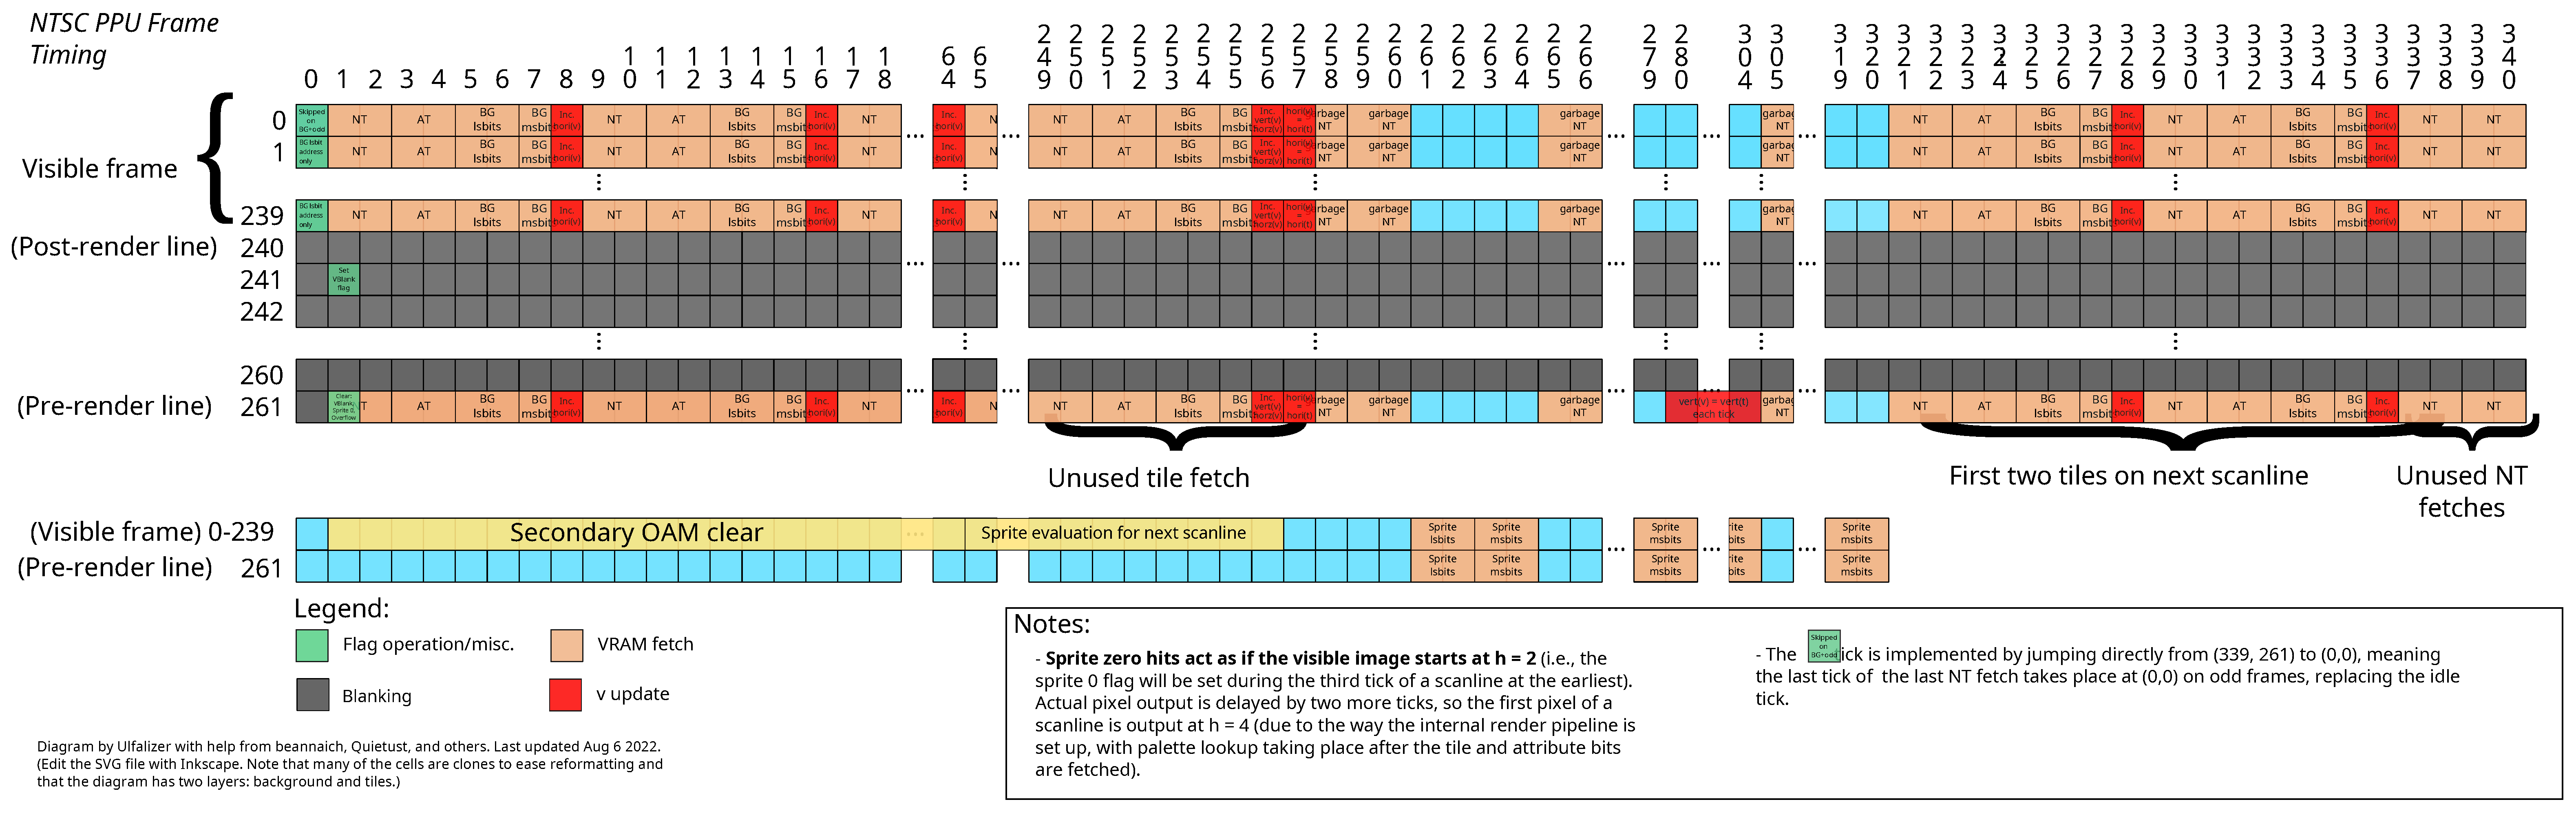
\includegraphics[width=1\textheight, angle=270]{images/ppudiag.pdf}
\end{figure}

\chapter
\begin{figure}[p!]
	\centering
	\caption{Přehledové hardwarové schéma konzole NES. Obrázek \enquote{NES-001 Console} vytvořil schenkzoola pod licencí CC~BY~4.0.}
	\label{fig:nes001-hw}
	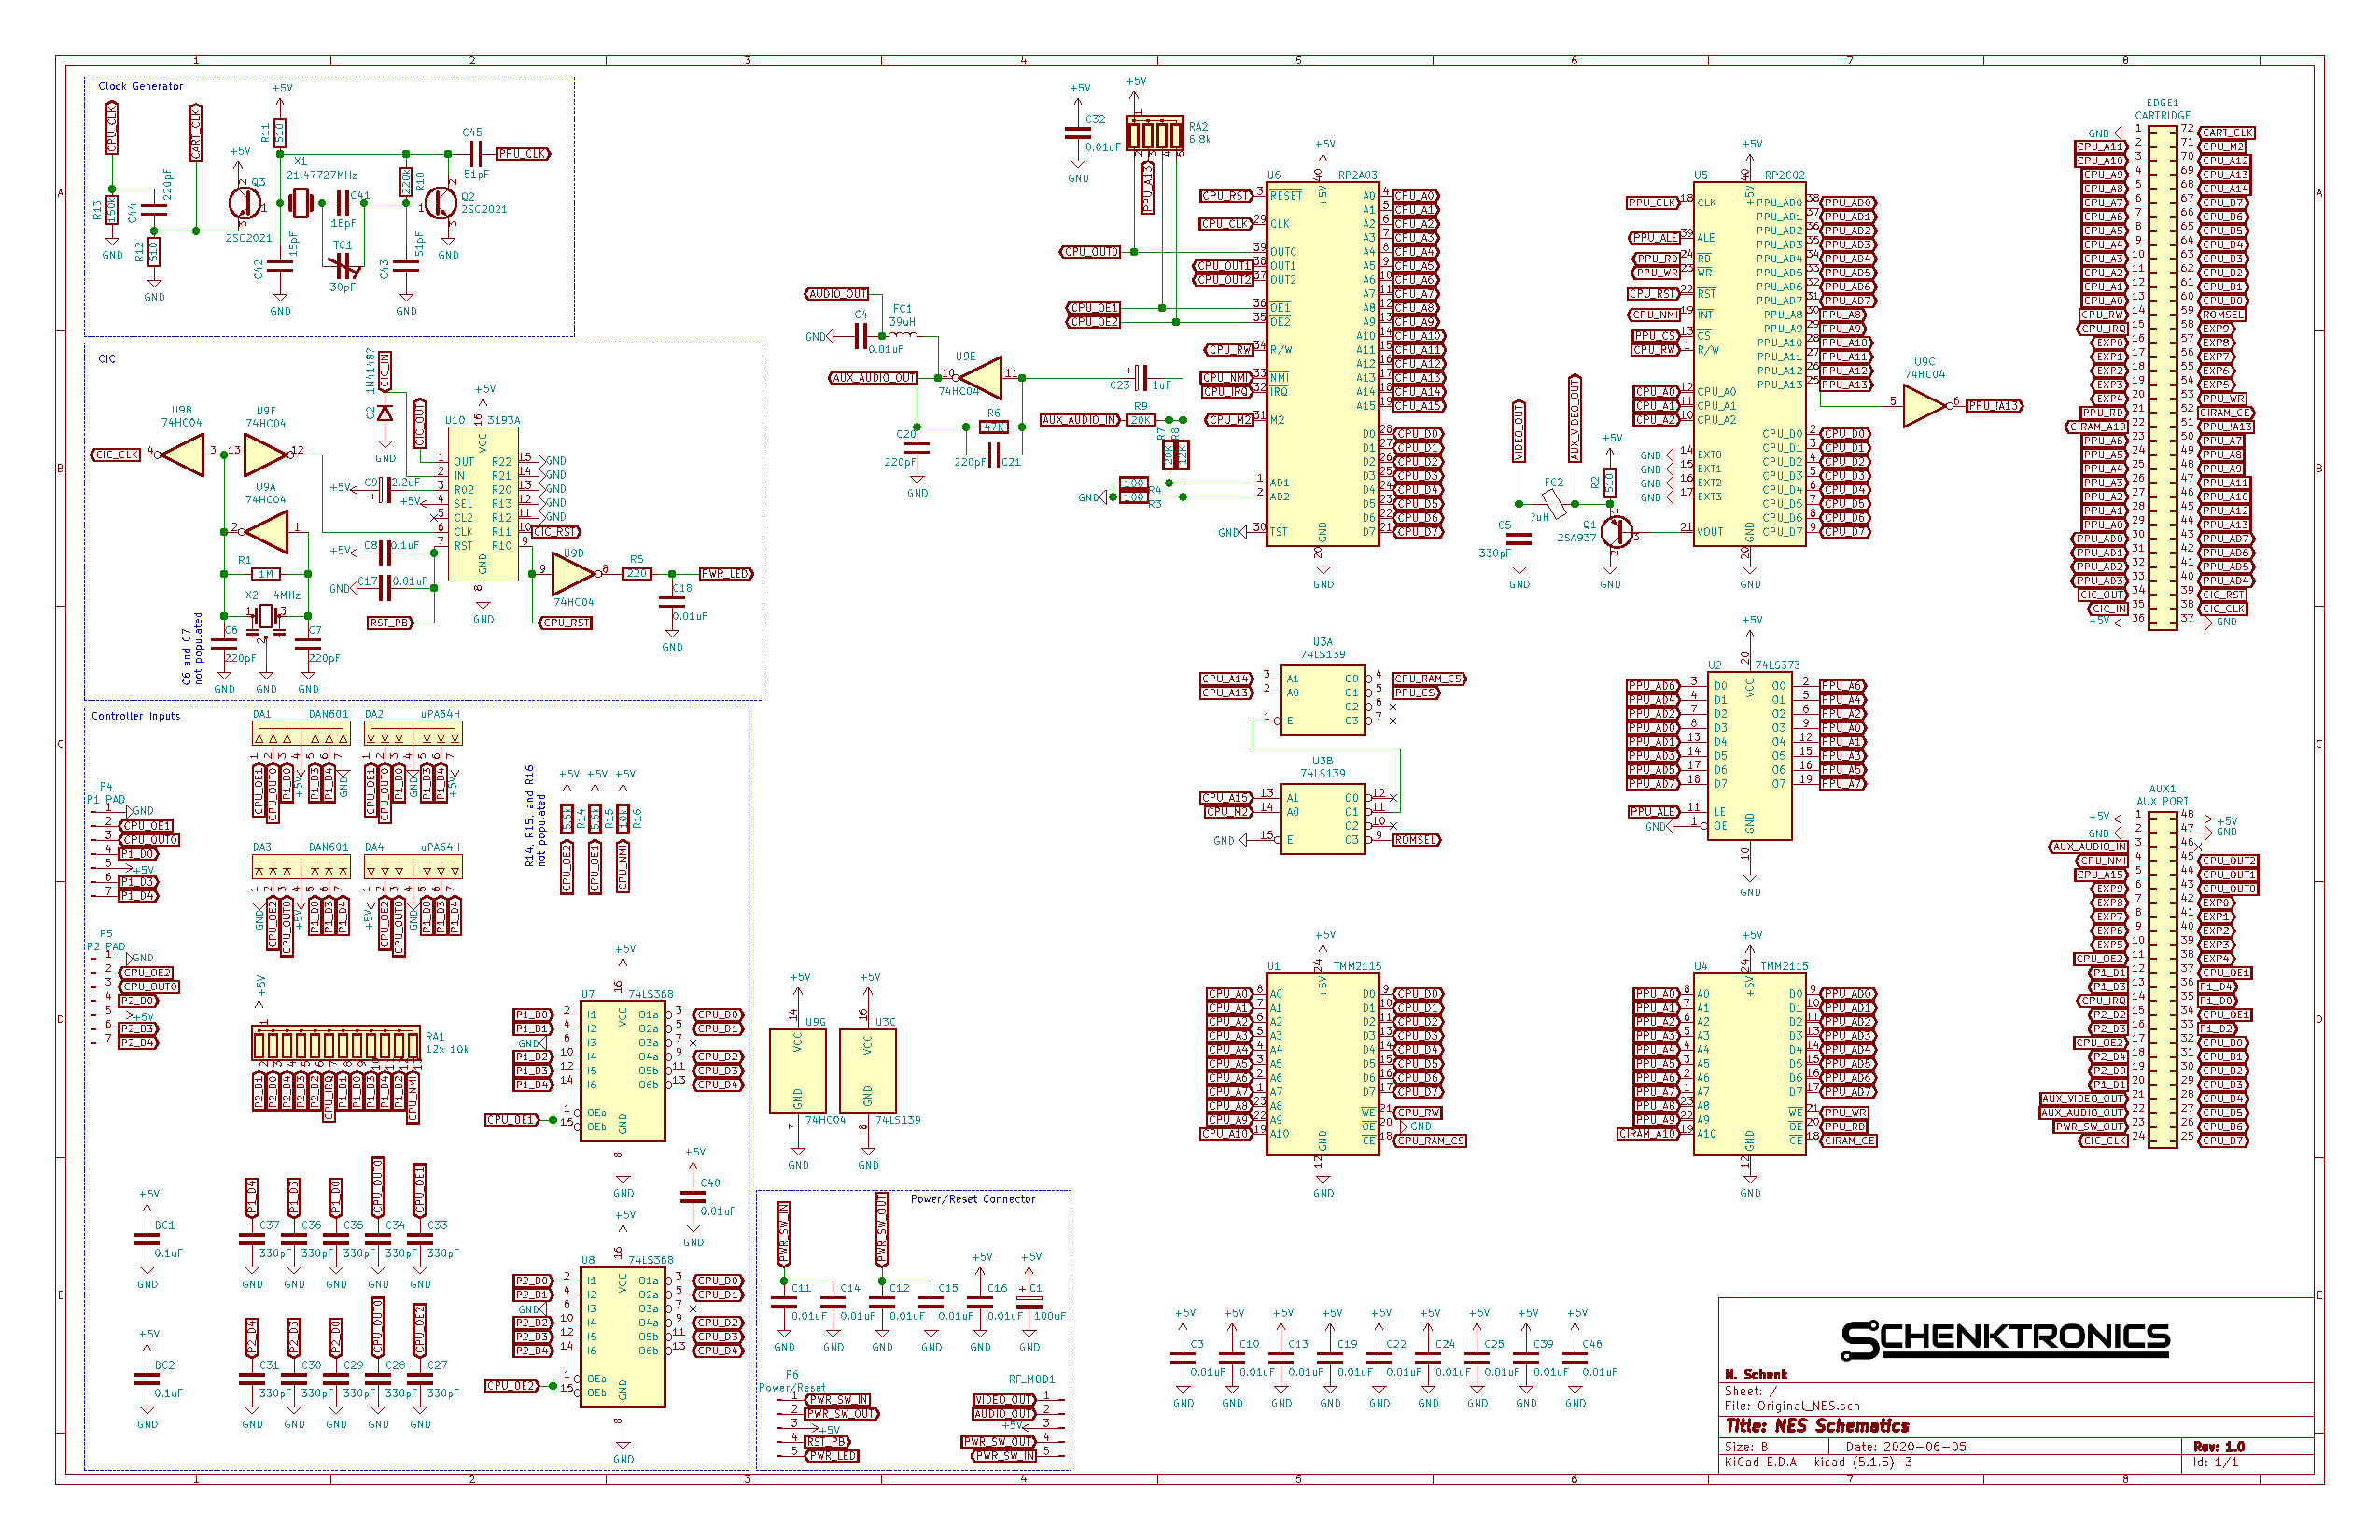
\includegraphics[width=0.95\textheight, angle=270]{images/NES-001.pdf}
\end{figure}

\chapter{Knihovna ImInputBinder}
\label{apx:binder}

Knihovna ImInputBinder vznikla jako rozšíření pro projekt Universal System Emulator.


